\documentclass{beamer}
\usepackage{graphicx}
\usepackage{tikz}
\usepackage{mathtools}
\usepackage{ragged2e}
\usepackage{adjustbox}
\title{The Hyperedge Event Model}
\author{\textbf{Bomin Kim}\\ \vspace{0.25cm} Department of Statistics\\Pensylvania State University}
\date{July 29, 2018\\\vspace{0.5cm} Joint Statistical Meetings 2018}
\begin{document}
\maketitle
\begin{frame}
		\frametitle{Collaborators}
		\hspace{0.5cm}
		\begin{figure}
								{
\includegraphics[width=.3\textwidth]{aaron.jpg}}
			{\includegraphics[width=.2245\textwidth]{Bruce.jpeg}}
				{\includegraphics[width=.3\textwidth]{Hanna.jpeg}}
		\end{figure}
\begin{itemize}
	\item \textcolor{blue}{Aaron Schein}\\\footnotesize{College of Information and Computer Sciences, UMass Amherst}
	\normalsize
	\item \textcolor{blue}{Bruce Desmarais}\\\footnotesize{Department of Political Science, Pennylvania State University}
\item		\normalsize\textcolor{blue}{Hanna Wallach}\\ \footnotesize{Microsoft Research NYC}	\normalsize
		\end{itemize}
\end{frame}
\begin{frame}
		\frametitle{Motivations: \textcolor{red}{H}yperedge \textcolor{red}{E}vent \textcolor{red}{M}odel}
		\normalsize	\begin{itemize}
			\item \textcolor{red}{H}\textcolor{blue}{yperedge}: directed edges from one sender to multiple receivers or from multiple senders to one receiver\vspace{0.15cm}
			\item \textcolor{red}{E}\textcolor{blue}{vent}:
			timestamped events in the continous-time scale\vspace{0.15cm}
			\item  \textcolor{red}{M}\textcolor{blue}{odel}: statistical framework to jointly understand\\\vspace{0.15cm}
		\end{itemize}
		\centering\Large
		``who interacts with whom, and when?"
\end{frame}

\begin{frame}
	\frametitle{Generative Process: ``\textcolor{red}{Who} Interacts with \textcolor{red}{Whom}"}
For event $e = 1,\ldots, E,$ between $i \in \{1,\ldots,A\}$ \& $j \in \{1,\ldots,A\}$,\normalsize\vspace{0.15cm}
	\begin{itemize}
		\item \textcolor{blue}{Receiver intensity} for every sender-receiver pair $(i, j)_{i\neq j}$
		\begin{equation*}
		\lambda_{iej} = \boldsymbol{b}^T \boldsymbol{x}_{iej},
		\end{equation*}
		where $\boldsymbol{x}_{iej}$ is a set of receiver selection features or covariates and $\boldsymbol{b}$ is the corresponding $P$-dimensional coefficient. \vspace{0.15cm}
		\item Every sender $i$ selects \textcolor{red}{candidate receivers} from non-empty \textcolor{blue}{multivariate Bernoulli distribution}\footnote{\scriptsize Fellows and Handcock (2017); Dai et al. (2013)} $\boldsymbol{u}_{ie} \sim \mbox{MB}_G ({\lambda}_{ie1},\ldots, {\lambda}_{ieA})$
				\begin{equation*}
			P(\boldsymbol{u}_{ie}|\boldsymbol{b}, \boldsymbol{x}_{iej}) \propto \exp\Big(\log(I(||\boldsymbol{u}_{ie}||_1 > 0))+\sum_{j\neq i} \lambda_{iej}u_{iej}\Big)
				\end{equation*}
	\end{itemize}
	
\end{frame}
\begin{frame}
	\frametitle{Generative Process: ``and \textcolor{red}{When}"}
		\begin{itemize}
			\item \textcolor{blue}{Timing rate} for each sender $i$
			\begin{equation*}
			\mu_{ie} = g^{-1}(\boldsymbol{\eta}^T \boldsymbol{y}_{ie}),
			\end{equation*}
				where $\boldsymbol{y}_{ie}$ is a set of timing features or covariates and $\boldsymbol{\eta}$ is the corresponding $Q$-dimensional coefficient. \vspace{0.15cm}
			\item \textcolor{blue}{Generalized linear model} (GLM) for time increment $\tau_{ie}$ so that
			\begin{equation*}
			E(\tau_{ie}) = 	\mu_{ie} \mbox{ and } V(\tau_{ie}) = V(	\mu_{ie}),
			\end{equation*}
			with a choice of distribution from exponential family.\vspace{0.15cm}
			\item Select the sender-receiver-set with \textcolor{blue}{the smallest time increment}\footnote{\scriptsize Snijders (1996)}
						\begin{equation*}
						\begin{aligned}
						s_e &= \mbox{argmin}_{i}(\tau_{ie}),\\
						\boldsymbol{r}_e &= \boldsymbol{u}_{s_e e},\\
						t_e &=t_{e-1} + \tau_{s_e e}.
						\end{aligned}
						\end{equation*}
		\end{itemize}
	\end{frame}
	\begin{frame}
		\frametitle{Generative Process: \textcolor{red}{Sender}, \textcolor{red}{Receivers}, and \textcolor{red}{Timestamps}\footnote{\scriptsize Assuming $t_{e-1}=0$ for simplicity.}}
					\begin{figure}[H]
						\centering
						\includegraphics[width=1\textwidth]{diagramnew.png}	
						\label{figure:diagram}
					\end{figure}
				\normalsize
					\begin{itemize}
						\item \textcolor{blue}{Bayesian inference}: invert the generative process to obtain the posterior
distribution over the latent variables---i.e., ($\boldsymbol{u},\boldsymbol{b},\boldsymbol{\eta})$.
					\end{itemize}						
			\end{frame}
			
				\begin{frame}
			\frametitle{Application: Montgomery County Government
\textcolor{red}{Email} Data\footnote{\scriptsize ben Aaron et al. (2017)}}
\begin{itemize}
	\item Email corpora covering inboxes and outboxes of \textcolor{blue}{Montgomery county government managers} in North Carolina \vspace{0.15cm}
	\item Contains \textcolor{blue}{$E=680$} emails, sent and received by \textcolor{blue}{$A=18$} department managers over 3 months (March--May) in 2012.\vspace{0.15cm}
			\end{itemize}
					\centering\Large``To what extent are \textcolor{blue}{nodal, dyadic or triadic network effects} relevant to predicting future emails?"
					
		\end{frame}				
		\begin{frame}
			\frametitle{Results: Exploratory Analysis on \textcolor{red}{$\boldsymbol{b}$}}
					\begin{equation*}
	\mbox{logit}(\lambda_{iej})=\log\Big(\frac{\lambda_{iej}}{1-\lambda_{iej}}\Big) =b_{1}+b_{2} x_{iej2}\ldots+b_{14}x_{iej14},\normalsize
					\end{equation*}
						\begin{figure}[!t]
						\centering
								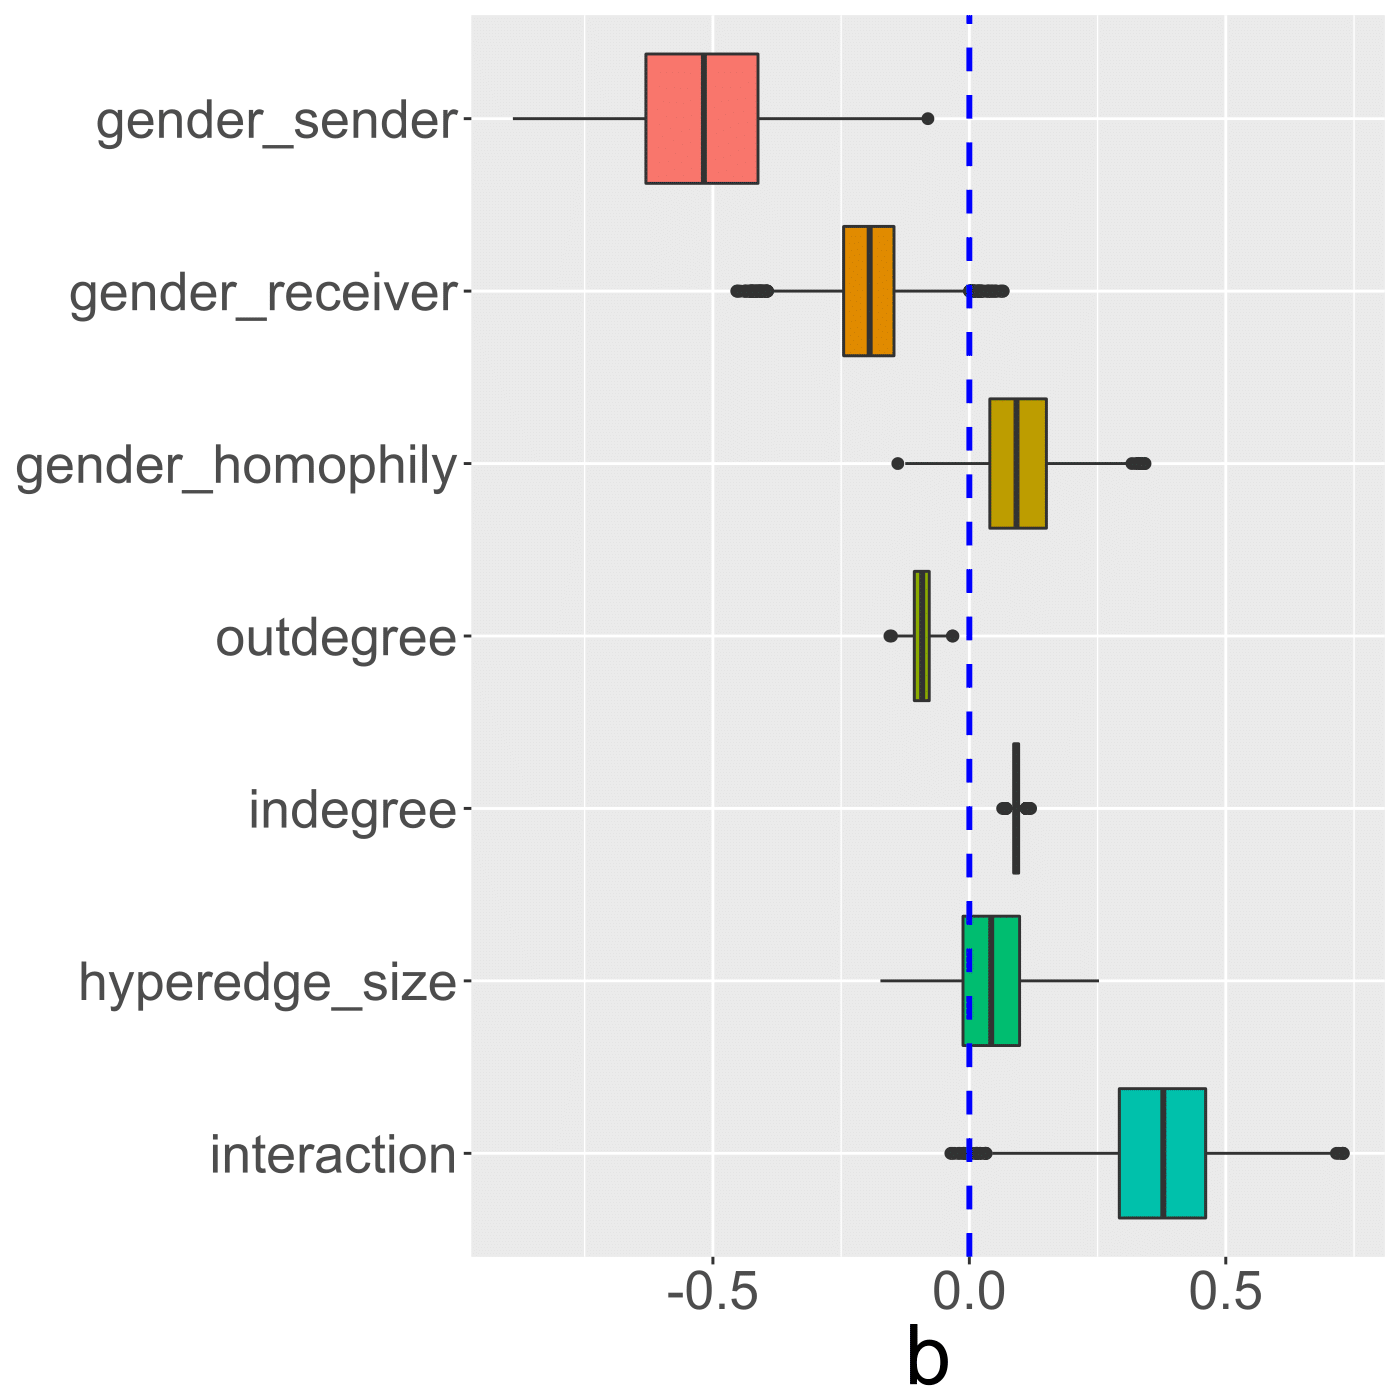
\includegraphics[width=0.45\textwidth]{betanewplot2-1.png}
								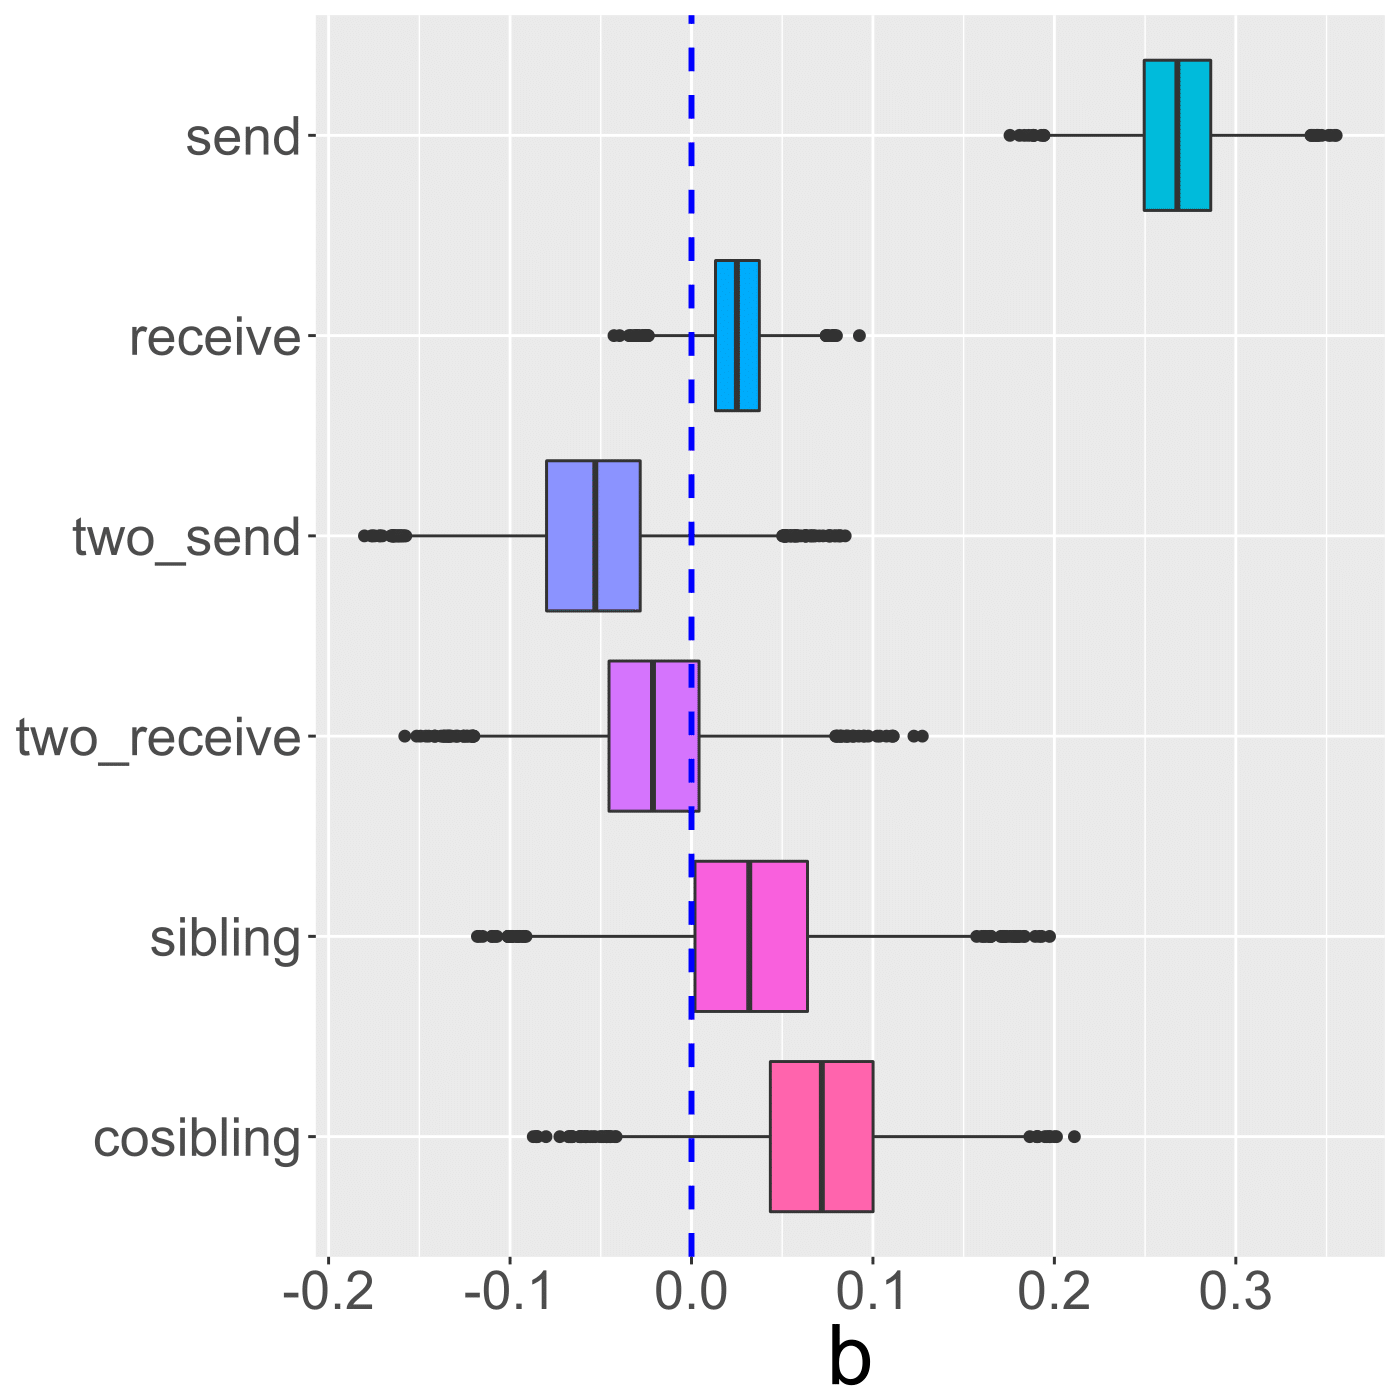
\includegraphics[width=0.45\textwidth]{betanewplot3-1.png}
					\end{figure}
					\begin{itemize}
						\item Log odds is two times less if the sender is a woman.\vspace{0.15cm}
						\item If $i$ sent $n$ number of emails to $j$ last week, then $i$ is $e^{0.27n} \approx (1.32)^n$ times more likely to send an email to $j$.
					
					\end{itemize}				
		\end{frame}	
		
				\begin{frame}
					\frametitle{Results: Exploratory Analysis on \textcolor{red}{$\boldsymbol{\eta}$}}
					\begin{equation*}
					\begin{aligned}
					&\log(\tau_{ie}) \sim N(\mu_{ie}, \sigma_\tau^2), \mbox{ with }
\mu_{ie} = \eta_{1}+\eta_{2} y_{ie2}\ldots+\eta_{7}y_{ie7}.
					\end{aligned}
					\normalsize
					\end{equation*}
			\begin{figure}[H]
				\centering
				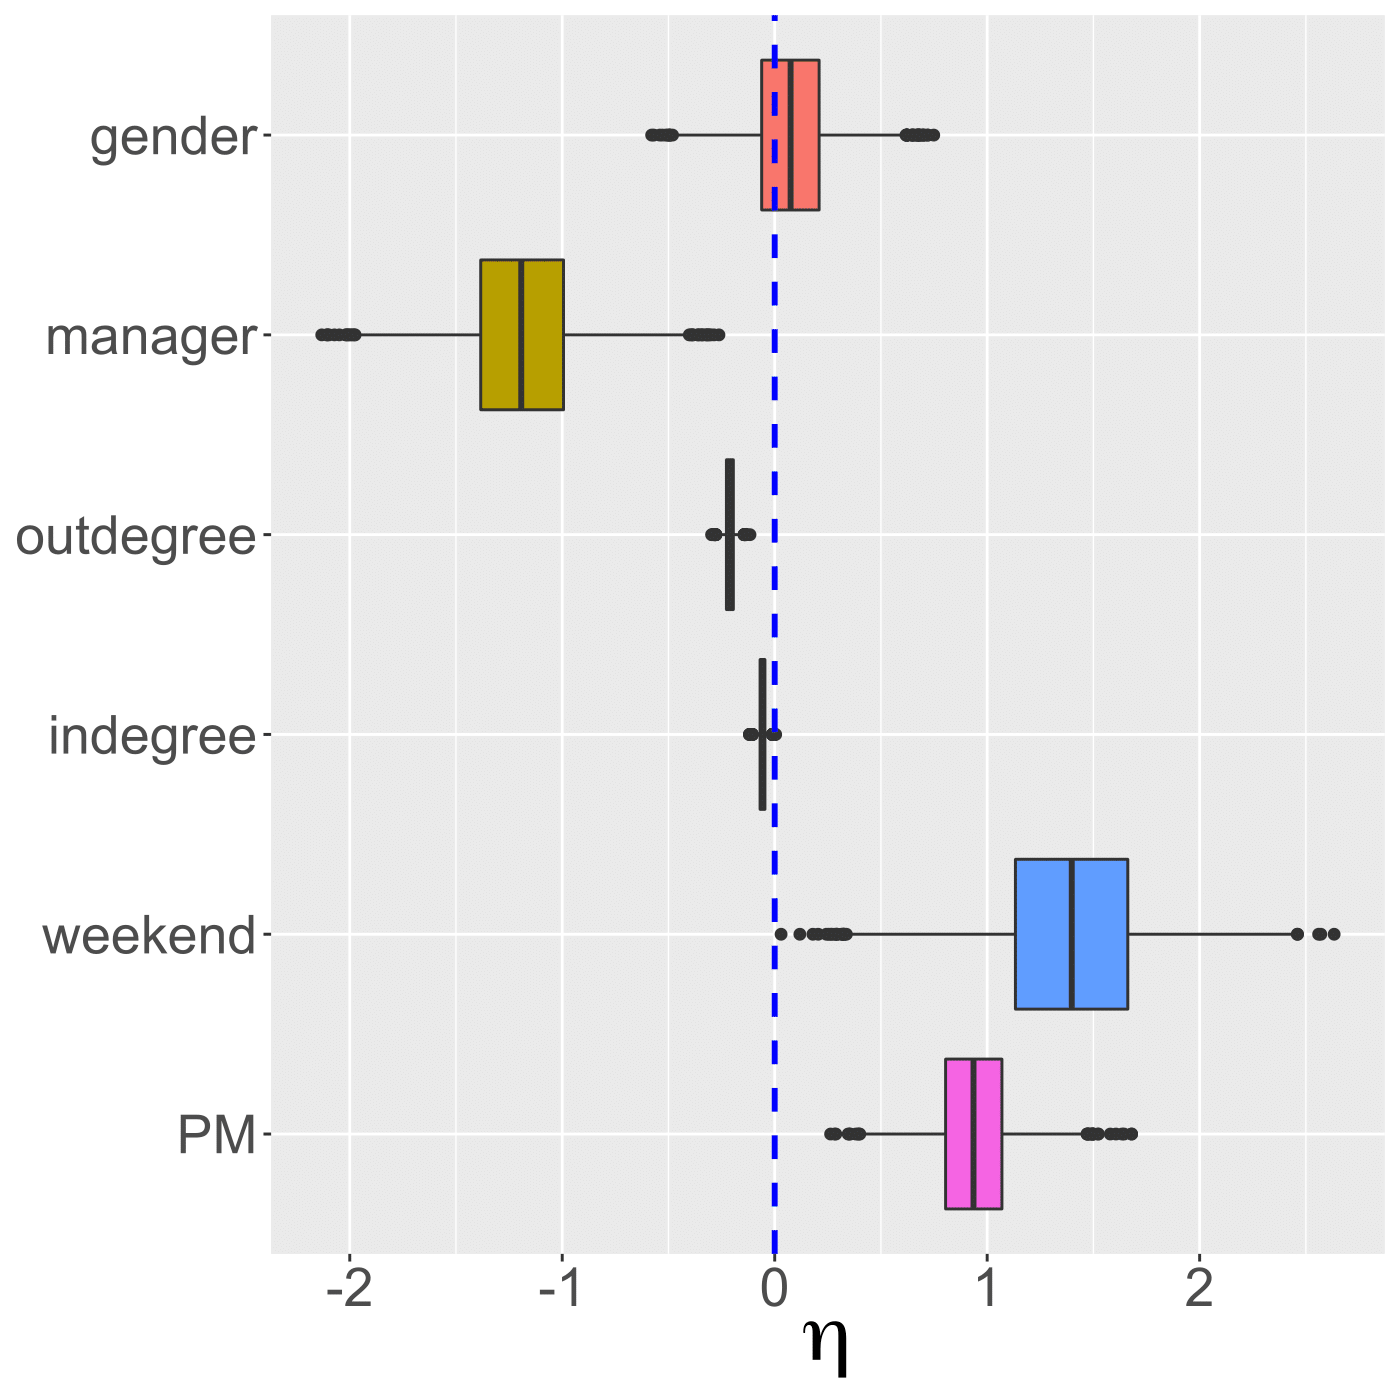
\includegraphics[width=0.45\textwidth]{etaplotnew-1.png}	
			\end{figure}	
								\begin{itemize}
						\item If an email was sent during weekend or PM, then time
						to next email takes $e^{1.55} \approx 4.72$ and $e^{0.98}\approx 2.67$
hours longer.\vspace{0.15cm}
						\item manager, outdegree, and indegree shorten time to next email.						
					\end{itemize}				
				\end{frame}				
				
							
				\begin{frame}
					\frametitle{Comparison: \textcolor{red}{Lognormal} vs. \textcolor{red}{Exponential}}
					\begin{itemize}
						\item \textcolor{blue}{Out-of-sample predictions}: sender, receiver, and timestamp 
							\begin{figure}[!t]
								\centering
										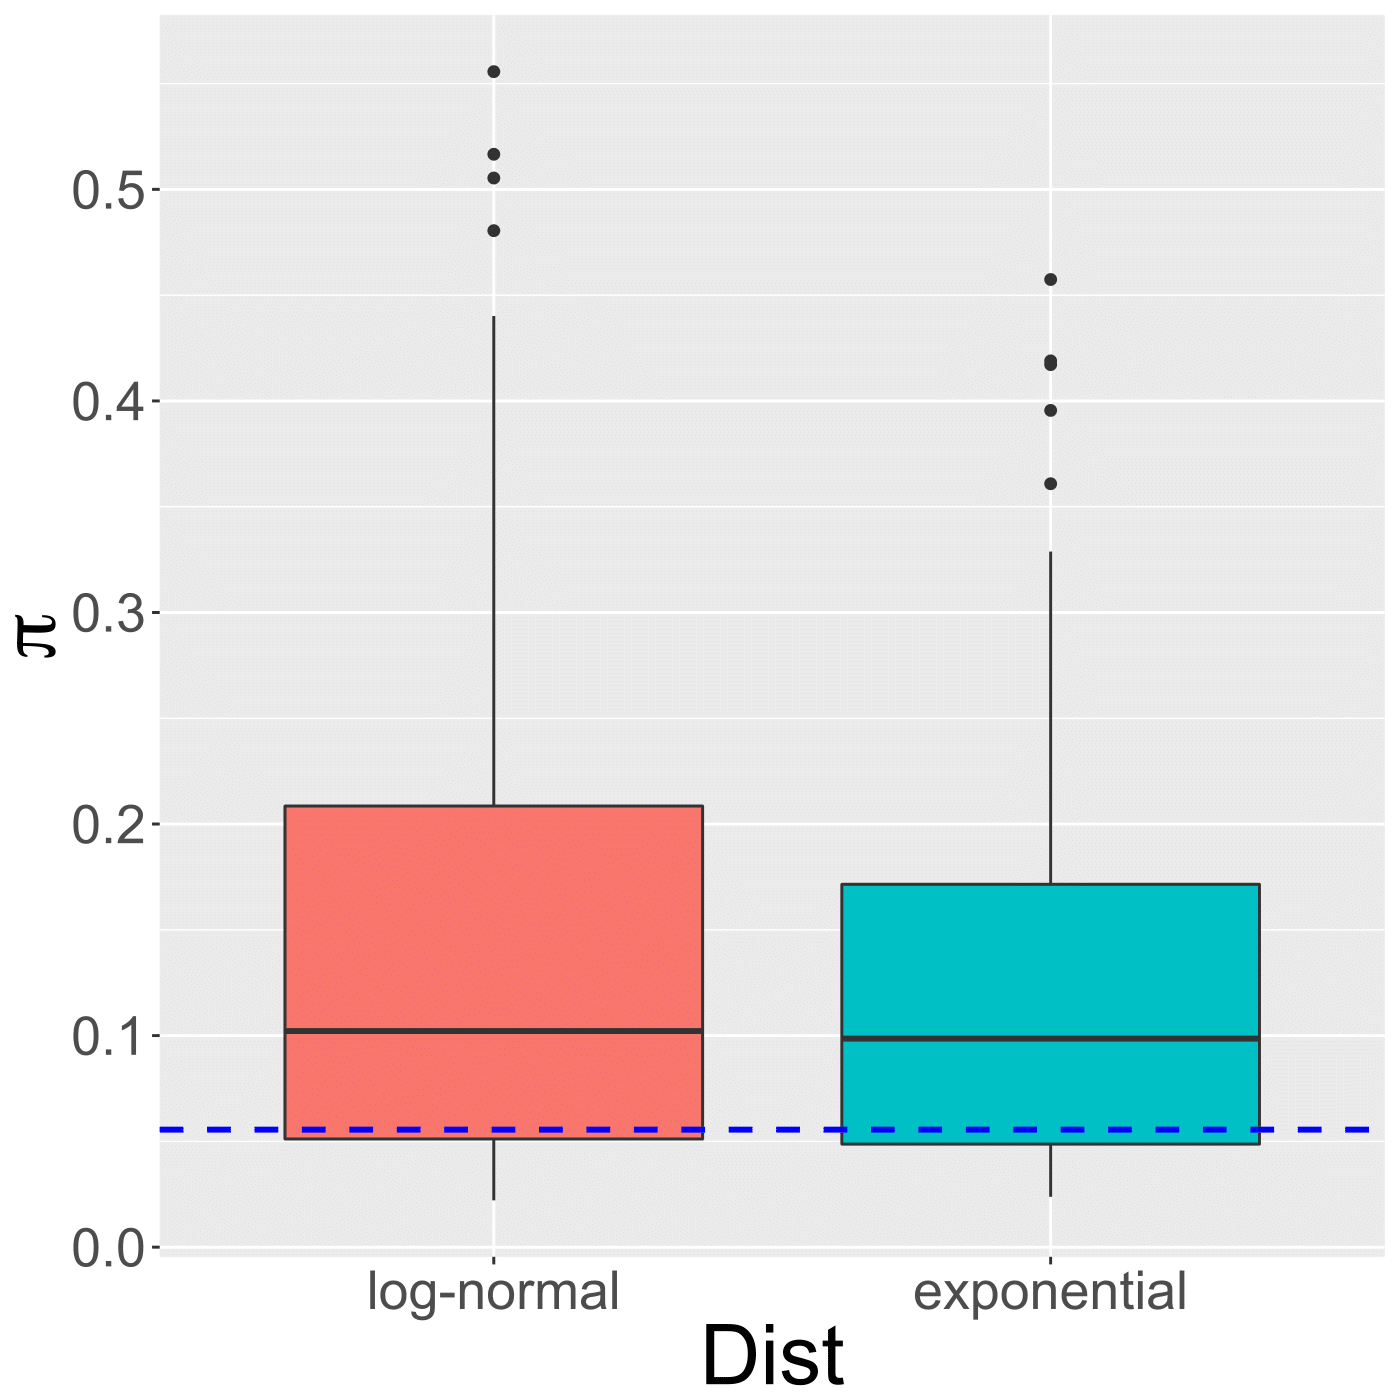
\includegraphics[width=0.3\textwidth]{senderpredict-1.png}	
										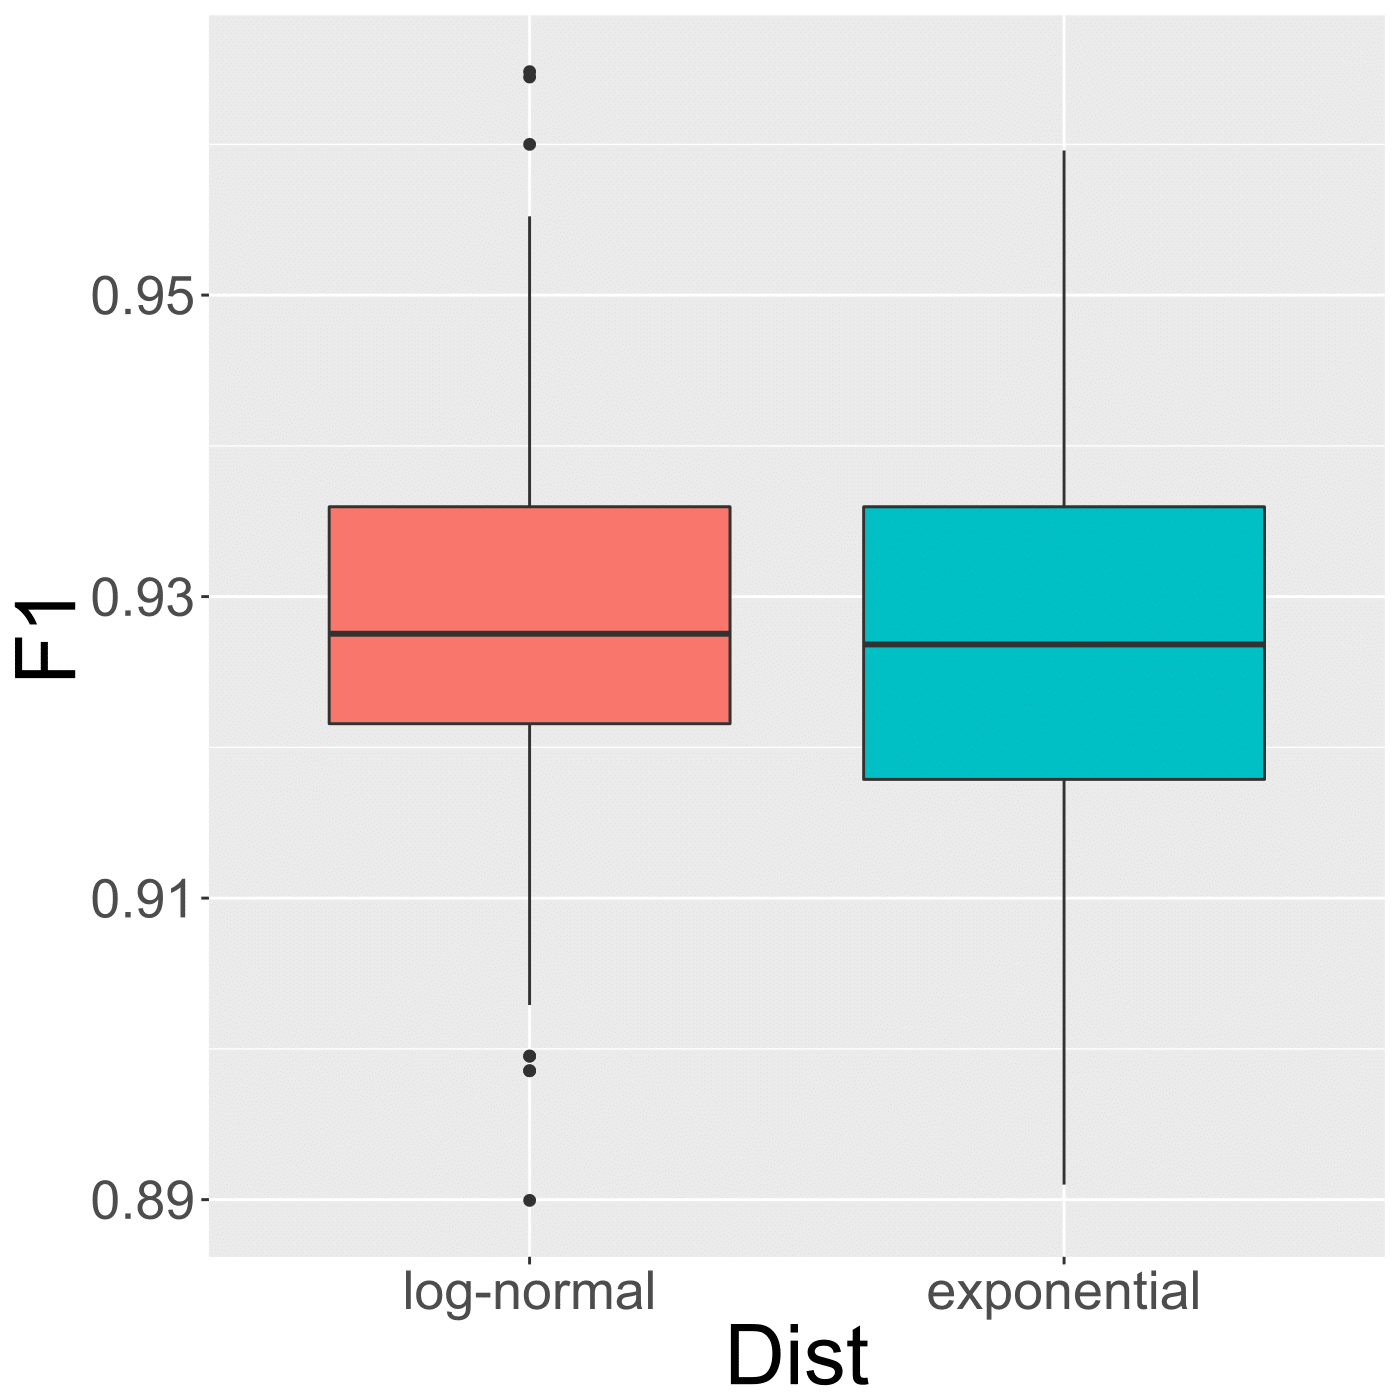
\includegraphics[width=0.3\textwidth]{receiverpredict-1.png}	
										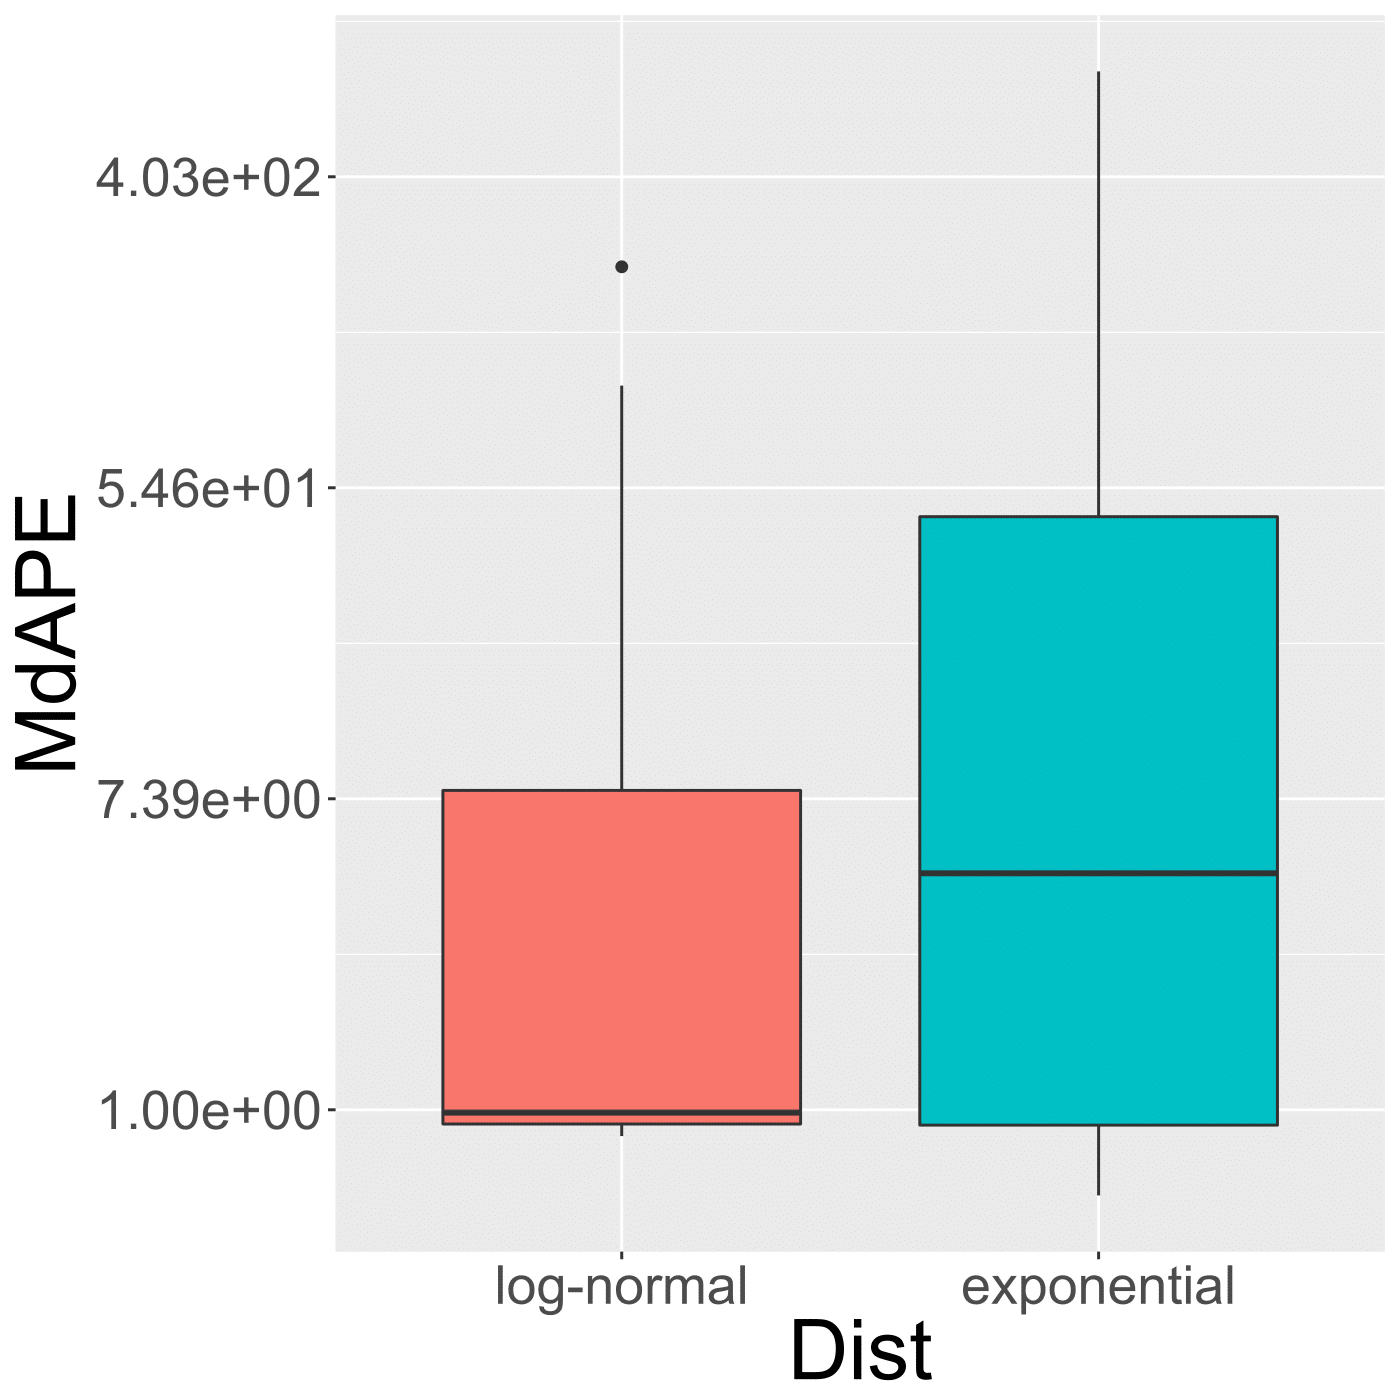
\includegraphics[width=0.3\textwidth]{timepredict-1.png}
							\end{figure}		
							
						\item \textcolor{blue}{Posterior predictive checks} (PPC)
							\begin{figure}[t]
								\centering
										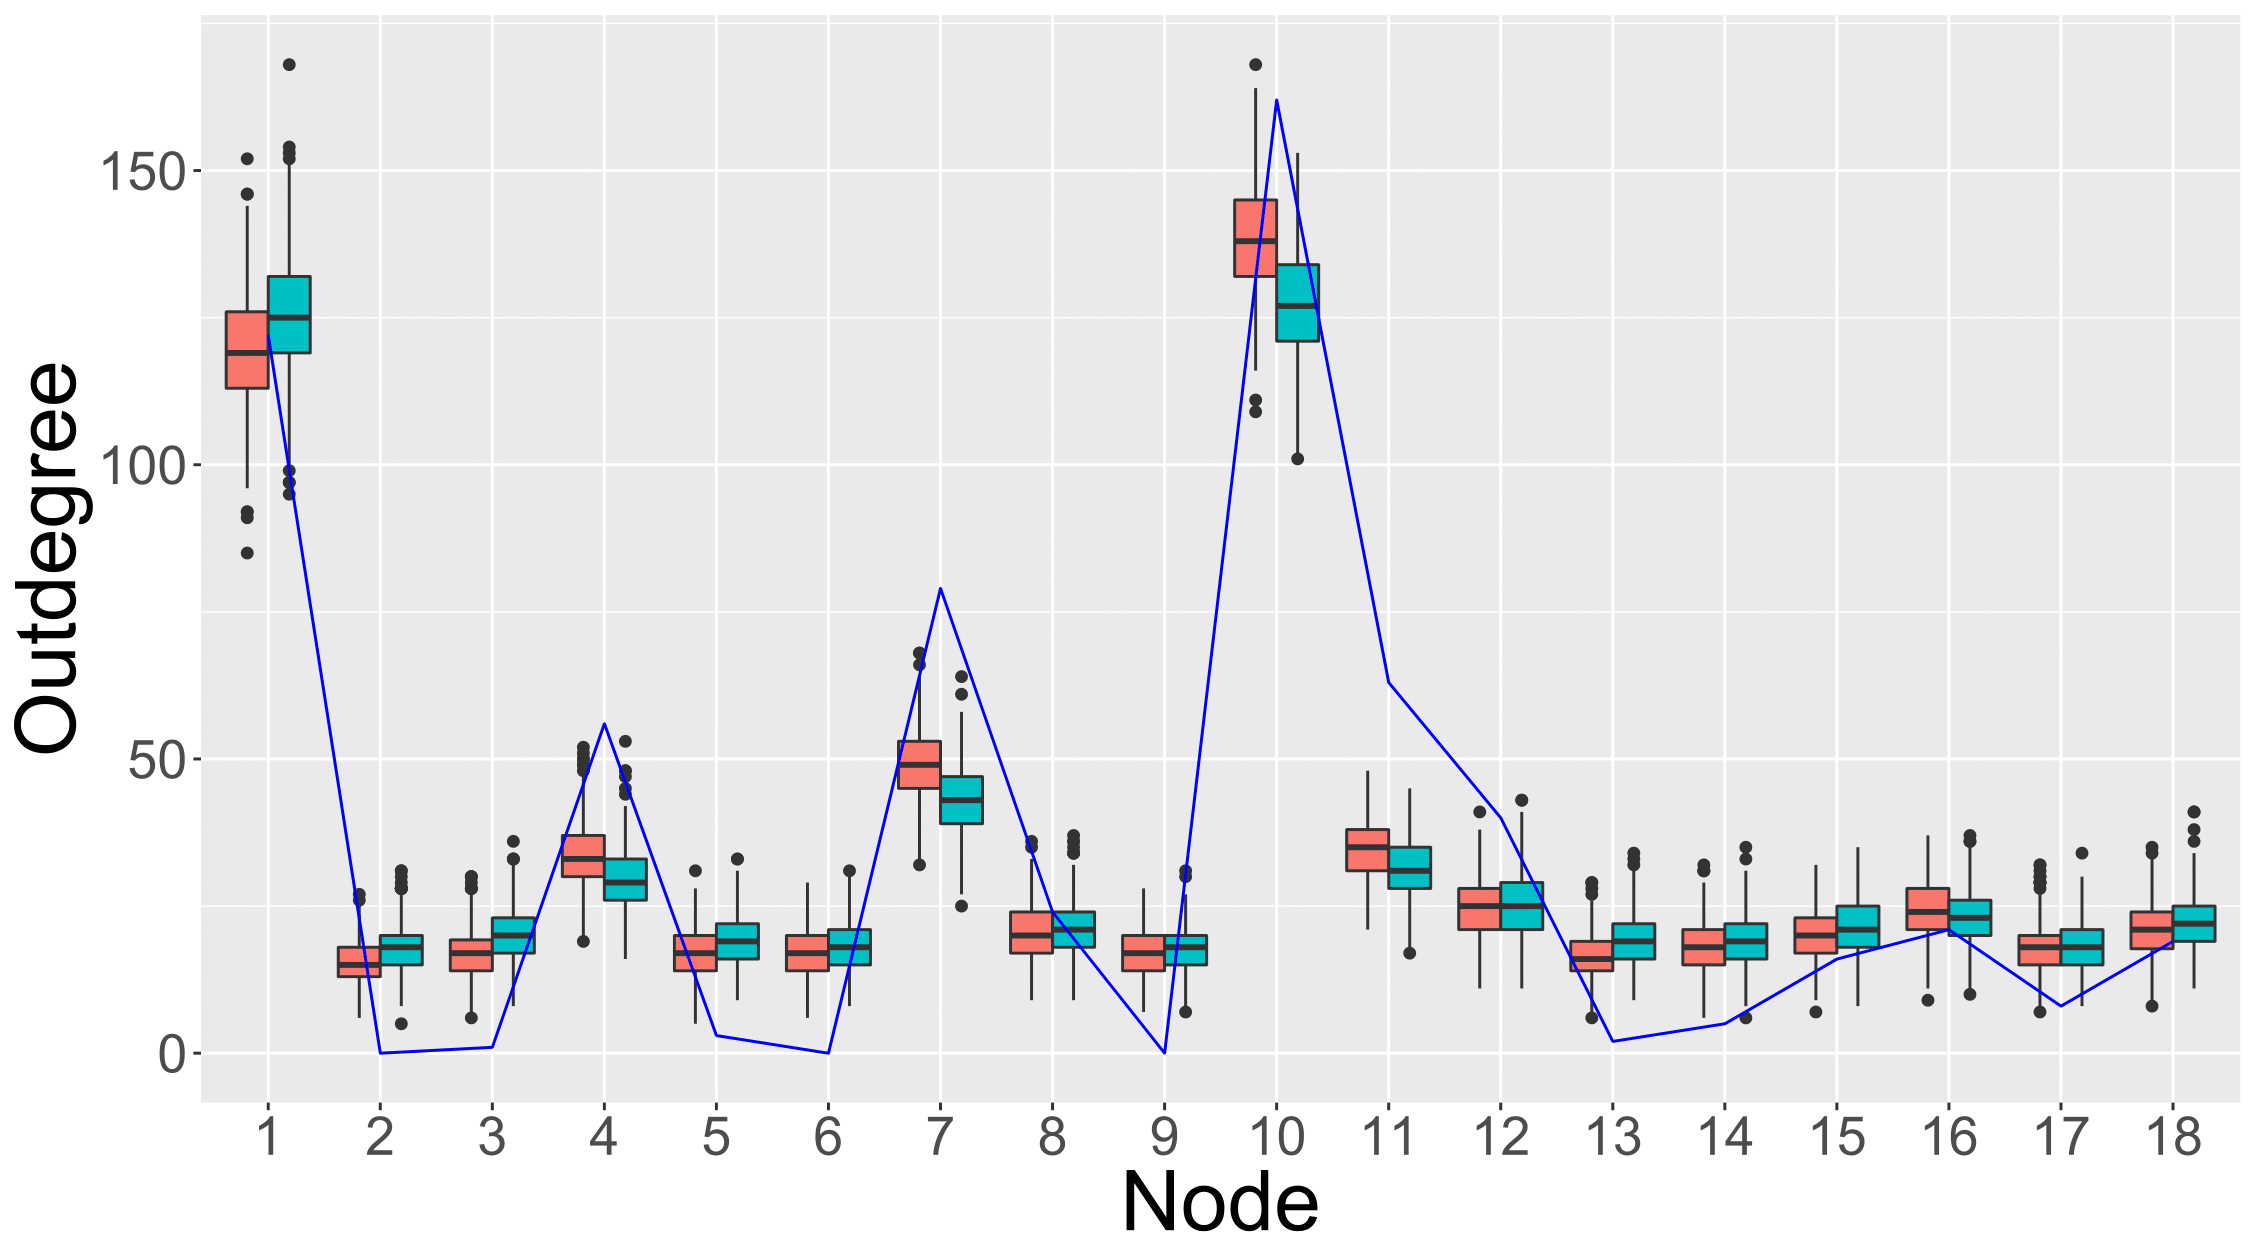
\includegraphics[width=.54\textwidth]{outdegree2-1.png}	
										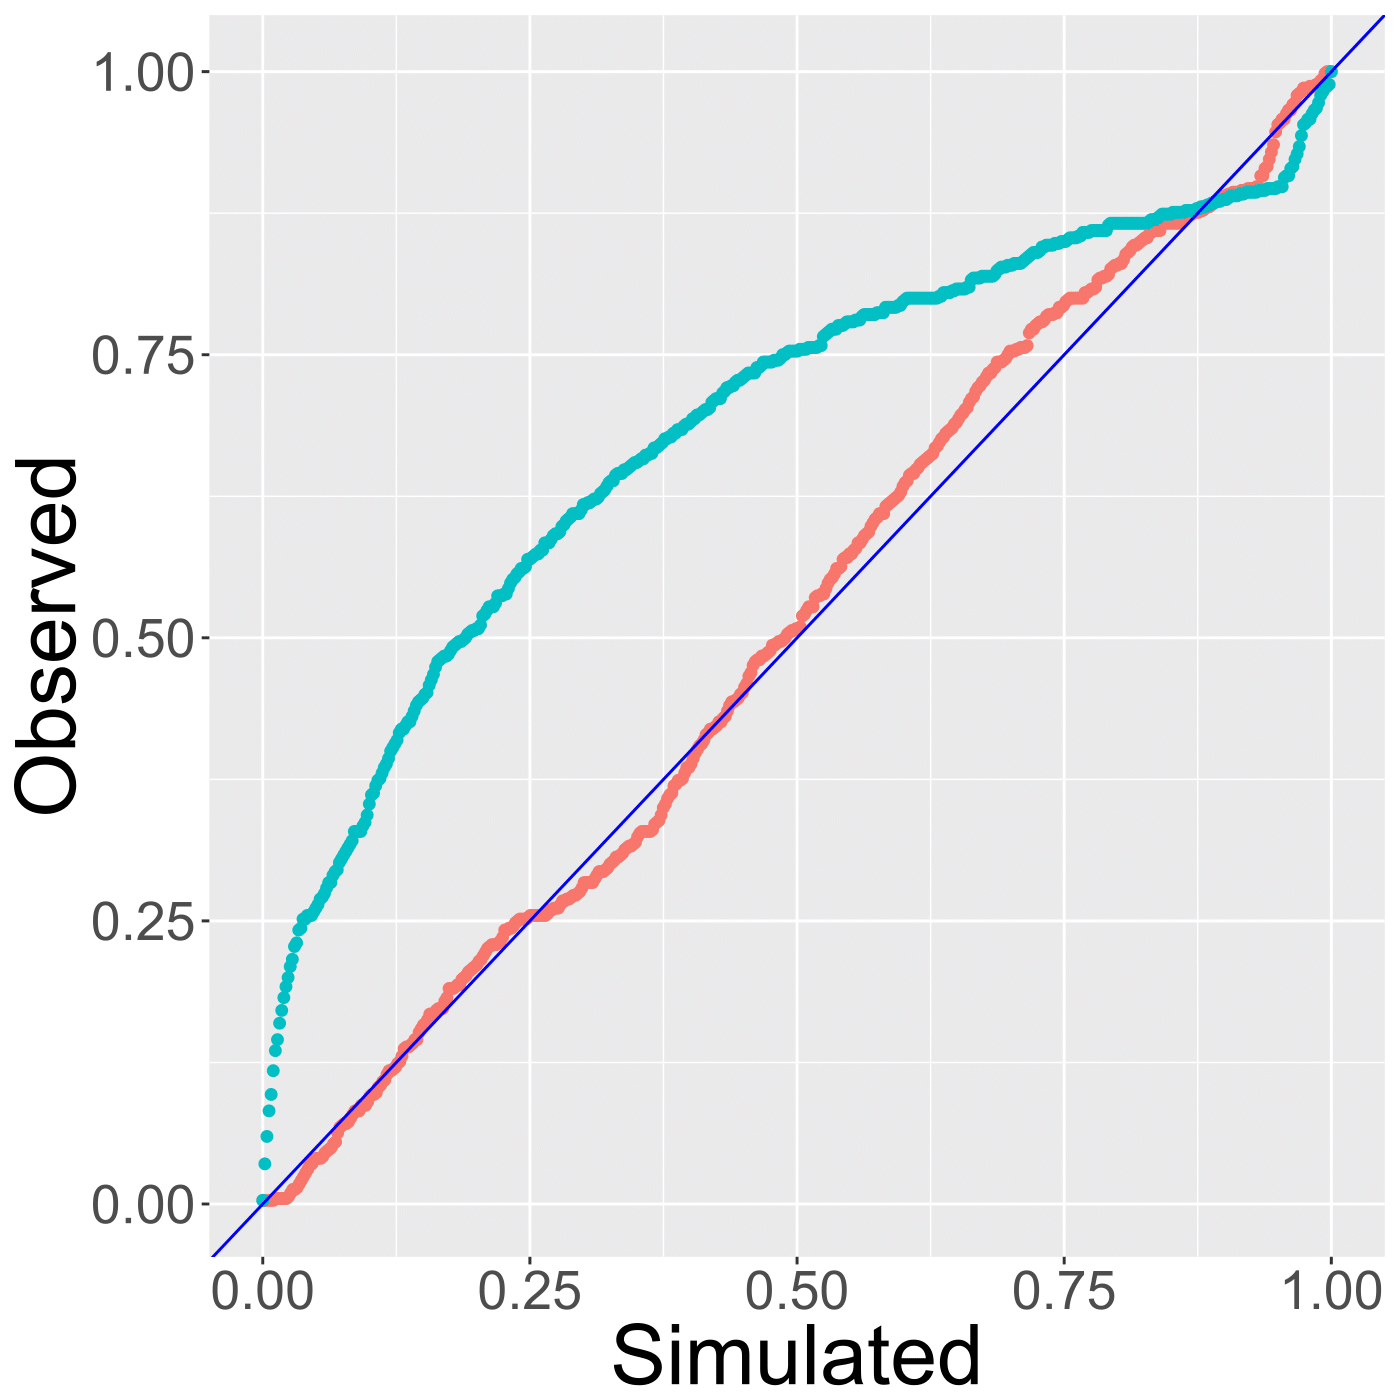
\includegraphics[width=0.3\textwidth]{timePPplot2-1.png}
							\end{figure}
							
					\end{itemize}
				\end{frame}	
							\begin{frame}
								\frametitle{Conclusion and Discussion}
								\begin{itemize}
									\item Account for \textcolor{blue}{hyperedges} without duplications\vspace{0.15cm}
									\item Flexible choice of \textcolor{blue}{continuous-time distribution} via GLM\vspace{0.15cm}
									\item Reverse the process for  \textcolor{blue}{multiple senders to one receiver}\\ (e.g., international sanctions and co-sponsorship of bills)\vspace{0.15cm}
									\item Sources: http://arxiv.org/abs/1807.08225 \\
						https://github.com/desmarais-lab/MulticastNetwork
									
								\end{itemize}
							\end{frame}	
							
\end{document}